% !TEX root = DesignDocument.tex


\chapter{System and Unit Testing Design}
\label{ch:testing}

% This section describes the approach taken with regard to system and unit testing.    This chapter does not describe the outcome of those tests.    

\section{Overview}
The testing approach is based on manual testing so far. 
The website and file conversion are tested separately, with their integration being tested as well.
Our tests ensure that the features provided in our user stories are met and work as intended.
The tests for each user story can be found below.

\section{Dependencies}
The main testing framework for the Azure website is Microsoft's C\# testing framework. 
The file conversion needs no external testing framework as it is tested manually for accuracy.

\section{Test design and setup}
There are currently no unit tests for the website, as all testing has been done by hand so far.
We may utilize Microsoft's C\# testing framework in the future. There is currently a testing project setup for the website but there are no tests currently available in it.
The file conversion testing is performed manually, as we cannot validate accuracy of conversion through software alone. We have a variety of files that we have tested through our development that we've used to show we can convert from one format to another.

\begin{itemize} \item Upload Maple 3D file to a cloud server \end{itemize}
\hspace{7mm}    
    Tested by manually accessing the website and uploading a file, then checking that it is present in the filesystem.

\begin{itemize} \item Maple 3D file will be automatically converted to a QR tag \end{itemize}
    \hspace{7mm}
    This feature is not yet implemented, but the conversion test was tested manually as a part and the as a system with the website.

\begin{itemize} \item Download the QR tage for a model from the cloud server \end{itemize}
    \hspace{7mm}
    Tags for models are not yet available, but a user can download a converted version of their uploaded file.

\begin{itemize} \item View the QR tage with an AR headset and render the 3D model \end{itemize}
    \hspace{7mm} 
    QR tags are not yet implemented, but we successfully rendered 3D models on the hololens by accessing files through OneDrive or using the converted file from the upload page.

\begin{itemize} \item Convert a 3D file from one format to another 
    \end{itemize}
    \hspace{7mm}
    The file conversion is manually tested using a variety of inputs to ensure robust and consistent performance. As there are two libraries (assimp and FBX SDK), they were both manually tested for simple functionality as the were implemented. After the two were put together, we had more tests to run. We tried sending through file types that can be inputs for assimp and made sure that the file made it to the FBX section and output the correct file format (.fbx). There are many different inputs so we sent through files for the common types we would expect such as .stl, .obj, .dae etc. Unsupported file types were also tested and we received appropriate errors from the conversion libraries. The file types supported for our system are available in Table \ref{tab:suportedfiletypes}. We also tried large files so we would know how long we could expect the system to take to process files of different sizes. There are certain limitations on the HoloLens hardware for file size and complexity that can be rendered, so we are aware of the limitations on that end and will inform our users appropriately. 
    
    We also tested files with textures embedded in them, to make sure the textures get converted with the file. With the file types we tried such as .obj and .fbx, the textures converted with the files as expected. The default 3d file viewer in the HoloLens currently does not support colors or textures, so we have not been able to test these features on the HoloLens yet. 

    The test files we ran through our system came from a variety of sources. We had a simple sphere generated in Maple as a .stl file, which we successfully converted through our system to .fbx to view on the HoloLens. We also received a .fbx representing a column, sent to us from a mathematics professor. The website \url{http://free3d.com} has many 3d files of varying formats and we ran some of them through our system. Sample files included a car, building, space ship, Batman, and other unique files. These files were available as .fbx and were good for testing out the HoloLens, but usually other formats came with them that we could convert them to .fbx as well. Lastly, we received some sample architectural files from one student's family member that were drawings of large buildings in .fbx format. One of these files rendered in the HoloLens, but the other two were too large to render because they exceeded the mesh/vertex limit for the viewer. This was when we looked into the limitations of the built in viewer.

    An example of converting a file through our system can be seen below in Figures \ref{Car-FBX}, \ref{Car-OBJ}, and \ref{Car-STL}. 
    We found a 3d file for a car online in the FBX format. 
    Our system then converted it to an OBJ format, as the File Converter software determined it only needed the FBX SDK to convert from FBX $\rightarrow$ OBJ. 
    The third model is an STL file generated from the FBX file, using a DAE file as an intermediate format between the FBX SDK and assimp libraries. 
    As is apparent in Figure \ref{Car-STL} below, the STL file does not contain the colors or smooth surfaces that are present in the other file types, and this is a limitation of the STL file format. 
    This system works for converting STL $\rightarrow$ FBX as well, but the colors would not be present in the final file because that information is not contained in the STL. 
    The STL format is one that can be exported from Maple software.

\begin{itemize} \item All other user stories post MVP are not yet implemented or tested, and they pertain mostly to secure accounts, file permissions, and more advanced features on the HoloLens viewer. 
These features will be tested appropriately through manual testing or the C\# framework as they are developed. \end{itemize}

\begin{figure}[H]
    \centering
    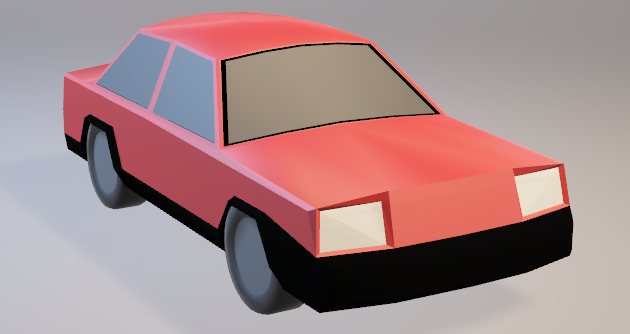
\includegraphics[width=\textwidth]{Car-FBX.png}
    \caption{Car FBX File}
    \label{Car-FBX}
\end{figure}

\begin{figure}[H]
    \centering
    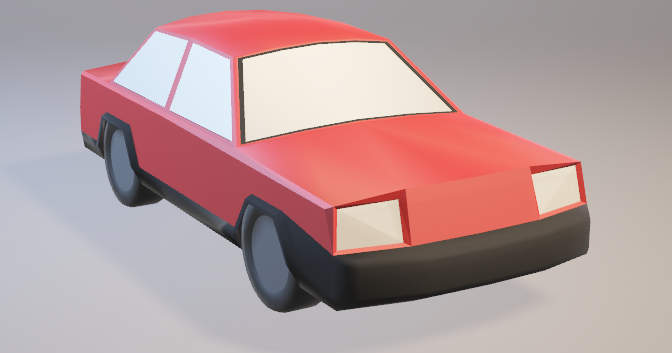
\includegraphics[width=\textwidth]{Car-OBJ.png}
    \caption{Car OBJ File}
    \label{Car-OBJ}
\end{figure}

\begin{figure}[H]
    \centering
    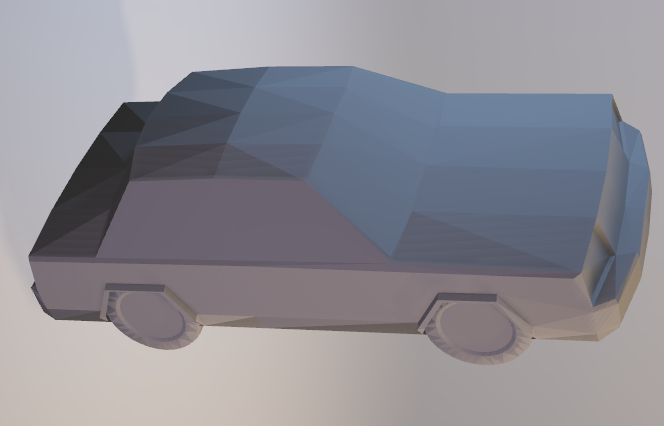
\includegraphics[width=\textwidth]{Car-STL.png}
    \caption{Car STL File}
    \label{Car-STL}
\end{figure}

\section{System Testing}
Testing our system involved manually using our software as a user would.
The test relied on being able to access the website, uploading a file, and being able to download the converted version of it.
This was successfully tested through manual tests and these features were present in our MVP.

\section{System Integration Analysis}
We performed some manual tests while integrating the file conversion with the website.
The integration was relatively simple and required us only to upload the executable to Azure and call it as we regularly would from our PC.
We successfully uploaded, converted, and downloaded files using the website to access the file conversion software.

\section{Risk Analysis}
There are two main risks associated with our project. These risks pertain to the functionality of the product itself and the security of our data.
Minimizing and preventing these risks are vital to providing quality software and positive relationships with users.

The first risk is that the software may fail to convert or render a given input file.
This could be caused by the file being too large or complex for our system to handle, or part of the file is corrupt. 

File security poses the other risk to our project, as some of the files uploaded may contain sensitive or confidential data.
We want to ensure that we maintain our users' privacy and trust as we strive to ensure only specified people can access certain files.
\subsection{Risk Mitigation}
To mitigate these risks, we have multiple strategies implemented to prevent the issues from happening in the first place.

Addressing the first risk of failed conversion or rendering, we will ensure product quality through rapid iteration and testing of MVPs. 
We have a variety of test files of varying sizes and formats that we have run through our system to make sure we cover many of the common (and uncommon) use cases.
Additionally, we aim to stay informed on the documentation of the libraries and platforms we use in our software to make sure we understand the capabilities and limitations of the tools we are using.
Especially for the file conversion software, we have researched which file types can be run through the libraries and have implemented that functionality in our product and need to communicate to our users which file types are acceptable for our system. 

For the second risk of data security, we try our best to examine and remove any possible security holes in our data flow.
We will need to analyze the website code to limit file access only to properly-privileged users. 
We also plan to implement features such as https and end-to-end encryption to maintain data security on our connections.